% Generated by pysimcount.pffigure -- do not edit; regenerate instead.
% figure: B-order8-by-formula -- Every order-8 formula at measured r
% source: results/pf-thesis/results.json
% metric=t gatebase=ct merged
% seed=1 t=n template=simcount synth=pygridsynth
% git_commit=04cd66abb614bdc66fb48e891cef085a299e0ab1 git_dirty=False
% source_sha256=018e0b7603e6fc9f6ee358974f241415a3b93437700847b033937cc1d4250db8
% derived: B-order8-by-formula.tex restyled by pysimcount.figuniform: extrapolated points (r from power-law fit) drawn in their series' measured style, style-key legend entries removed; extrapolated n = [13, 20]; source_sha256=79a26b2dd7e2218448d395ea1b78721b6fa06430fa09b0c5924a2d371c26f58e
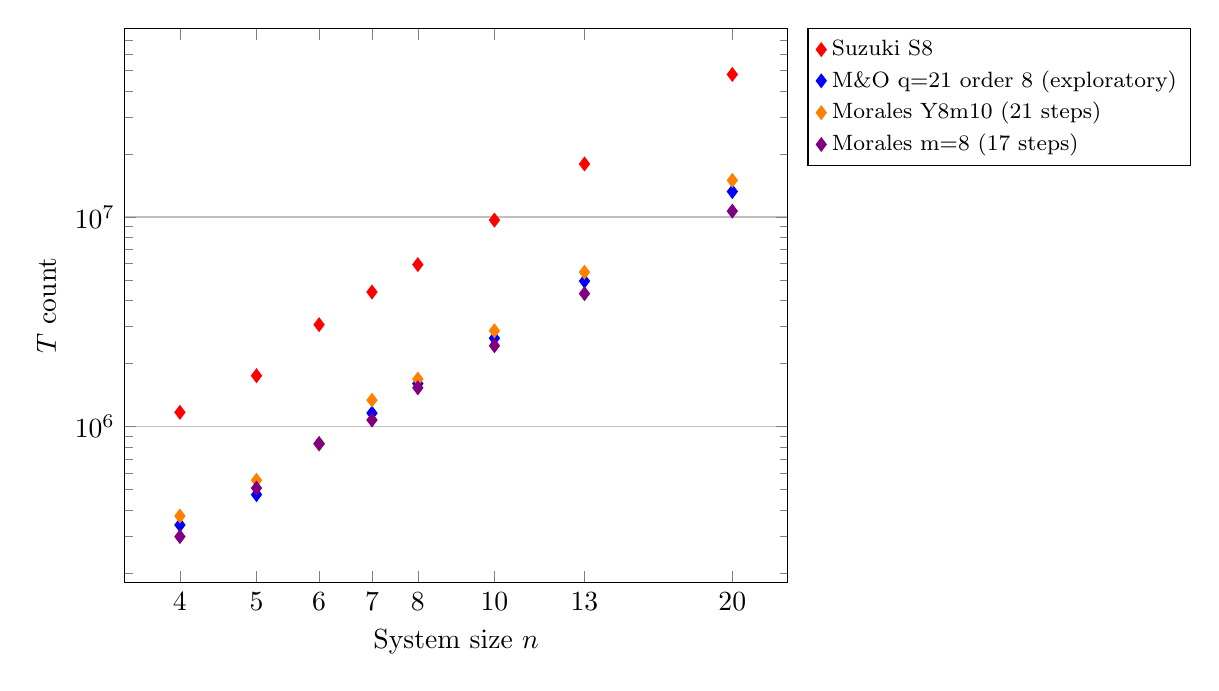
\begin{tikzpicture}
  \begin{loglogaxis}[
    width=10cm,
    xlabel={System size $n$},
    ylabel={$T$ count},
    xtick={4,5,6,7,8,10,13,20},
    xticklabels={4,5,6,7,8,10,13,20},
    ymajorgrids=true,
    legend pos=outer north east,
    legend cell align=left,
    legend style={font=\footnotesize},
  ]
    \addplot[only marks, red, mark=diamond*, mark size=2.4pt, mark options={solid, fill=red}] coordinates {
      (4,1168668)
      (5,1747718)
      (6,3063980)
      (7,4384584)
      (8,5927740)
      (10,9665928)
    };
    \addlegendentry{Suzuki S8}
    % r from power-law fit (extrapolation); one legend entry per series
    \addplot[only marks, red, mark=diamond*, mark size=2.4pt, mark options={solid, fill=red}, forget plot] coordinates {
      (13,17930450)
      (20,47957290)
    };
    \addplot[only marks, blue, mark=diamond*, mark size=2.4pt, mark options={solid, fill=blue}] coordinates {
      (4,338734)
      (5,472728)
      (6,825452)
      (7,1159000)
      (8,1603008)
      (10,2639650)
    };
    \addlegendentry{M\&O q=21 order 8 (exploratory)}
    % r from power-law fit (extrapolation); one legend entry per series
    \addplot[only marks, blue, mark=diamond*, mark size=2.4pt, mark options={solid, fill=blue}, forget plot] coordinates {
      (13,4947150)
      (20,13231134)
    };
    \addplot[only marks, orange, mark=diamond*, mark size=2.4pt, mark options={solid, fill=orange}] coordinates {
      (4,373992)
      (5,554064)
      (6,825520)
      (7,1336162)
      (8,1684400)
      (10,2865324)
    };
    \addlegendentry{Morales Y8m10 (21 steps)}
    % r from power-law fit (extrapolation); one legend entry per series
    \addplot[only marks, orange, mark=diamond*, mark size=2.4pt, mark options={solid, fill=orange}, forget plot] coordinates {
      (13,5456042)
      (20,14967520)
    };
    \addplot[only marks, violet, mark=diamond*, mark size=2.4pt, mark options={solid, fill=violet}] coordinates {
      (4,298080)
      (5,508064)
      (6,829206)
      (7,1074192)
      (8,1529304)
      (10,2429350)
    };
    \addlegendentry{Morales m=8 (17 steps)}
    % r from power-law fit (extrapolation); one legend entry per series
    \addplot[only marks, violet, mark=diamond*, mark size=2.4pt, mark options={solid, fill=violet}, forget plot] coordinates {
      (13,4307900)
      (20,10671120)
    };
  \end{loglogaxis}
\end{tikzpicture}
